\subfigure[Index notation $p$]  
{
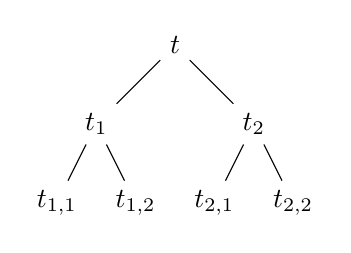
\begin{tikzpicture}
    \node (=) at (0,0){$t$};

    \node (+) at (-1,-1){$t_1$};
    \node (-) at (1,-1){$t_2$};
    \node (a) at (-1.5, -2) {$t_{1,1}$};
    \node (b) at (-0.5, -2) {$t_{1,2}$};
    \node (c) at (0.5, -2) {$t_{2,1}$};
    \node (d) at (1.5, -2) {$t_{2,2}$};

    \draw[] (=) -- (+);
    \draw[] (=) -- (-);
    \draw[] (+) -- (a);
    \draw[] (+) -- (b);
    \draw[] (-) -- (c);
    \draw[] (-) -- (d);
\end{tikzpicture}
}
\subfigure[Symbols $t_p$]  
{
\begin{tikzpicture}
    \node (=) at (0,0){$=$};
    \node (+) at (-1,-1){$+$};
    \node (-) at (1,-1){$-$};
    \node (a) at (-1.5, -2) {$a$};
    \node (b) at (-0.5, -2) {$b$};
    \node (c) at (0.5, -2) {$c$};
    \node (d) at (1.5, -2) {$d$};

    \draw[] (=) -- (+);
    \draw[] (=) -- (-);
    \draw[] (+) -- (a);
    \draw[] (+) -- (b);
    \draw[] (-) -- (c);
    \draw[] (-) -- (d);
\end{tikzpicture}
}
\subfigure[Sub-terms $T_p$]  
{
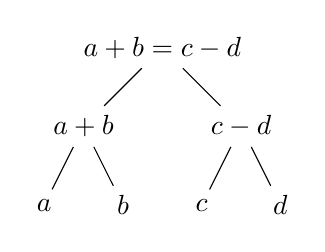
\begin{tikzpicture}
    \node (=) at (0,0){$a+b=c-d$};

    \node (+) at (-1,-1){$a+b$};
    \node (-) at (1,-1){$c-d$};
    \node (a) at (-1.5, -2) {$a$};
    \node (b) at (-0.5, -2) {$b$};
    \node (c) at (0.5, -2) {$c$};
    \node (d) at (1.5, -2) {$d$};

    \draw[] (=) -- (+);
    \draw[] (=) -- (-);
    \draw[] (+) -- (a);
    \draw[] (+) -- (b);
    \draw[] (-) -- (c);
    \draw[] (-) -- (d);
\end{tikzpicture}
}
\caption{
Example of the syntax tree for the term $a+b=c-d$ with maximal spread $s=2$.
To demonstrate the usage of position variable $p$ consider sub-figure (b) the tree with the concrete symbols and sub-figure (a) the same tree with the abstract $t_p$ notation side by side.
% the concrete symbols (a) and the here used notation $t_p$.
For comparison the tree in sub-figure (c) contains the sub-terms $T_p$.
}